%======================================================================
\section{Introduction}
%======================================================================
For a person with tetraplegia, an assistive robotic arm controlled by an intracortical
brain--computer interface (iBCI) could restore everyday manipulation: drinking from a
cup, eating, opening a door. Neuralink's CONVOY early-feasibility study
(NCT06710626)~\cite{neuralink2024convoy} pairs the N1 implant with an assistive robotic
arm. Academic iBCIs have already shown 3-D reach and grasp~\cite{hochberg2012reach},
7-DoF and 10-DoF control of an anthropomorphic arm~\cite{collinger2013high,wodlinger2015ten},
and tactile feedback that halves grasp times~\cite{flesher2021brain}.

Two problems separate these demonstrations from a product used every day.
\begin{enumerate}
\item \textbf{Decoding is noisy and drifts.} Even for the best decoders, offline R$^2$
  of attempted 7-DoF reach-and-grasp velocity from human motor cortex is around
  0.6--0.7~\cite{karpowicz2024falcon}. A decoder trained on one day degrades on the
  next~\cite{downey2018stability,jarosiewicz2015virtual,degenhart2020stabilization},
  so every session costs recalibration time.
\item \textbf{Decoding noise is fatal at the moment of grasp.} The last few centimetres
  and the gripper command are where BCI arm tasks fail~\cite{flesher2021brain,downey2016blending}.
  Shared autonomy, i.e.\ blending the user's command with a vision-guided autonomous
  policy, raised clinical grasp success from 22\% to 78\% for one participant in
  Downey et~al.~\cite{downey2016blending}. But it raises a safety and authority
  question: the robot must not keep moving toward the wrong object when the person
  changes their mind~\cite{dragan2013policy,javdani2015shared}.
\end{enumerate}

This paper builds and evaluates both halves end-to-end.
\begin{itemize}
\item \textbf{Multi-day 7-DoF decoding on real human data.} We use FALCON
  H1~\cite{karpowicz2024falcon}. We compare Wiener, Kalman, GRU and Transformer
  decoders with a \emph{multi-day GRU}: per-day linear read-ins and a shared recurrent
  core, recalibrated on a new day by fitting only a new read-in from seconds of data.
  We evaluate within session (FALCON's public minival split) and across 7 later days.
\item \textbf{Decoder-Aware Shared Autonomy (DASA).} The goal-inference likelihood is
  the decoder's own calibrated error model, fitted on the same open-loop calibration
  block as the decoder. It is corrected for the temporal autocorrelation of decoder
  errors and combined with a goal-switching prior and a consistency gate. DASA has no
  hand-tuned inference temperature.
\item \textbf{A simulated closed loop anchored to real data.} A delayed
  feedback-control user model~\cite{cunningham2011closed,willett2017feedback} drives a
  Poisson encoding model fitted to H1. Its spikes are decoded, arbitrated, and
  executed by a safety-filtered 7-DoF Kinova Gen3 kinematic model. We set the
  simulator's decoder quality so that its offline R$^2$ matches the real R$^2$ of the
  same decoder on the same session, then sweep it.
\end{itemize}

We compare DASA against decoder-only control, fixed blending, distance-based blending
(Downey~et~al.'s constants)~\cite{downey2016blending}, confidence-based policy
blending~\cite{dragan2013policy}, and hindsight-optimisation
assistance~\cite{javdani2015shared}. Results cover task success, time, path efficiency,
user authority, goal-inference accuracy, a change-of-mind scenario and a cluttered
scene, with paired statistics.

\paragraph{Scope.} The closed loop is \emph{simulated}; no person was in the loop. The
offline decoding results are on real data. All numbers come from runs of the
accompanying code; \S\ref{sec:repro} gives the full-scale configuration.

%======================================================================
\section{Background and related work}
%======================================================================
\paragraph{iBCI arm control.}
\begin{itemize}
\item BrainGate2~\cite{hochberg2012reach} decoded 3-D endpoint velocity with a Kalman
  filter~\cite{wu2006bayesian,kim2008neural} plus a discrete grasp classifier.
\item The Pitt group used optimal linear estimators to give one participant 7-DoF and
  then 10-DoF control of the Modular Prosthetic Limb~\cite{collinger2013high,wodlinger2015ten}.
  Path efficiency, however, stayed near 0.3--0.4~\cite{collinger2013high}.
\item Recurrent decoders~\cite{sussillo2012recurrent,sussillo2016making,deo2024brain}
  and pretrained Transformers~\cite{ye2021representation,ye2023neural,azabou2023unified,ye2025generalist}
  improve offline accuracy and cross-session robustness.
\item Sussillo et~al.~\cite{sussillo2016making} made RNN decoders robust by training on
  many days with synthetic nonstationarity.
\item Multi-session models align sessions through session-specific input layers. LFADS
  calls this ``stitching''~\cite{pandarinath2018inferring}; NDT2 and POYO use context
  tokens or unit embeddings~\cite{ye2023neural,azabou2023unified}.
\item Unsupervised alignment~\cite{degenhart2020stabilization,karpowicz2025stabilizing}
  and pseudo-labelling~\cite{wilson2025longterm,fan2023plug} avoid labelled
  recalibration altogether.
\item FALCON~\cite{karpowicz2024falcon} standardises few-shot cross-session evaluation.
  Its H1 task is the human 7-DoF reach-and-grasp data we use.
\end{itemize}

\paragraph{Shared autonomy.}
\begin{itemize}
\item \emph{Policy blending}~\cite{dragan2013policy} predicts the goal with maximum-entropy
  inverse optimal control (MaxEnt IOC)~\cite{ziebart2008maximum}. It arbitrates as
  $u=(1-\alpha)u_{\text{user}}+\alpha u_{\text{robot}}$, with $\alpha$ increasing in
  prediction confidence. Aggressive assistance helps when the prediction is right;
  timid assistance is better when it is wrong.
\item \emph{Hindsight optimisation}~\cite{javdani2015shared,javdani2018shared} treats
  the goal as latent in a POMDP and acts on the posterior-expected cost-to-go (QMDP).
  It can therefore assist before it is confident.
\item Learned copilots~\cite{reddy2018shared,lee2025copilots} and latent
  actions~\cite{losey2020controlling,jeon2020shared,losey2022learning} remove the need
  for a known goal set.
\item For iBCIs specifically:
  \begin{itemize}
  \item Muelling et~al.~\cite{muelling2017autonomy} combined object detection, MaxEnt
    goal inference and sigmoid arbitration.
  \item Downey et~al.~\cite{downey2016blending} blended BMI and robot velocities with an
    autonomy weight that is a sigmoid of distance to a vision-computed grasp pose.
  \item Lee et~al.~\cite{lee2025copilots} recently used AI copilots to enable
    pick-and-place with a non-invasive BCI.
  \end{itemize}
\item User acceptance depends on legibility and authority~\cite{brooks2020visualization,gopinath2017human}.
\end{itemize}
What these methods have \emph{not} exploited is that, in a BCI, the user's command is
the output of a decoder whose error statistics are measured during calibration. That
is the gap DASA addresses.

%======================================================================
\section{Data and decoding methods}
%======================================================================
\subsection{FALCON H1}
H1 (DANDI 000954~\cite{ye2024falconh1data}) contains open-loop calibration blocks from
one participant in the Pitt iBCI study. The participant attempted reach-and-grasp
movements while watching a virtual arm. The data are threshold crossings on 176
channels, binned at 20\,ms (we reproduce FALCON's binning exactly), and cued velocities
for 7 DoF:
\begin{itemize}
\item translation $t_x,t_y,t_z$;
\item wrist roll $r_x$;
\item three grasp dimensions $g_1$--$g_3$ (pinch, scoop, thumb abduction).
\end{itemize}

\paragraph{Splits.}
\begin{itemize}
\item \emph{Training:} 13 \emph{held-in} calibration blocks from 6 days (2{,}301\,s after removing the minival bins, see below). The
  last 15\% of each block is validation, used for all hyper-parameters and early stopping.
\item \emph{Within-session test:} FALCON's public \emph{minival} split, the later part of
  the same blocks.
\item \emph{Cross-session test:} FALCON's held-out evaluation data are private. We
  therefore use the 14 public \emph{held-out} calibration blocks, 7 days that are 6--20
  days after the last training day. On each day:
  \begin{itemize}
  \item block~A (about 48\,s) is the recalibration block; its first $k\in\{10,20,45\}$\,s
    of labels may be used;
  \item block~B, a separate later recording, is the test set.
  \end{itemize}
\end{itemize}

\paragraph{Train/test overlap in the public files.} Each public held-in \emph{calibration} file begins with exactly the bins of the corresponding \emph{minival} file; we verified this bin for bin for all 13 blocks. We strip these bins before training, and a unit test enforces it. In an earlier run that trained on the unstripped files, the GRU's held-in R$^2$ was 0.80, against \GRUWithin{} after stripping (\S\ref{sec:dec-results}). Anyone using minival for local evaluation should remove the overlap.

\paragraph{Metric.} We report FALCON's metric: R$^2$ computed per block over
\texttt{eval\_mask} bins with variance weighting across DoF, then averaged over blocks.
Variance weighting lets the large-variance grasp dimensions dominate, so we also report
per-DoF R$^2$ pooled over blocks.

Our held-out numbers are \emph{not} comparable to the FALCON leaderboard. Our held-in
numbers use the public minival split, not the leaderboard's test split.

\paragraph{Normalisation.} Spike counts are z-scored per day using that day's
calibration statistics. For held-out days, the statistics come from the
\emph{unlabelled} block~A, an unsupervised mean/variance tracking in the spirit
of~\cite{jarosiewicz2015virtual}. Velocities are z-scored with training statistics.

\subsection{Decoders}
\paragraph{Wiener filter.} This is FALCON's baseline. Ridge regression on lagged,
causally smoothed counts $\tilde r_t$ (exponential, $\tau=2$ bins):
\begin{equation}
\hat v_t=\sum_{k=0}^{L-1}W_k\,\tilde r_{t-2k}+b .
\end{equation}
Taps are spaced 40\,ms apart, so $L=15$ covers 600\,ms, matching FALCON's 30-bin
history. $L$ and the ridge strength are chosen on validation data.

\paragraph{Kalman filter.} The standard velocity Kalman filter~\cite{wu2006bayesian}:
\begin{equation}
x_t=Ax_{t-1}+w_t,\qquad y_t=Hx_t+h_0+q_t ,
\end{equation}
with steady-state gain. The least-squares $A$ is nearly the identity at 20\,ms and
integrates observation bias. A leaky $A=0.98I$ won on validation, and we report that.

\paragraph{GRU and causal Transformer.} The GRU is single-layer with 192 units on CPU.
The causal Transformer has 2 layers, width 128 and a 1\,s context.

\paragraph{Multi-day GRU (proposed decoder).}
\begin{equation}
h_t=\mathrm{GRU}\big(h_{t-1},\,\mathrm{drop}(R_d z_t+c_d)\big),\qquad \hat v_t=W_oh_t+b_o ,
\end{equation}
\begin{itemize}
\item One read-in $(R_d,c_d)$ per training day $d$ ($176\to64$); the core and readout
  are shared.
\item Training uses the nonstationarity augmentation of~\cite{sussillo2016making}:
  per-channel gain ($\sigma=0.1$ in log space), per-channel offset ($\sigma=0.1$) and
  5\% channel dropout.
\item \emph{Zero-shot} on a new day uses the mean read-in $\bar R$.
\item \emph{Few-shot}: we fit only a new read-in on the $k$ labelled seconds, with the
  core frozen and an anchor to $\bar R$:
\begin{equation}
\min_{R,c}\ \sum_t\big\|v_t-f_\theta(Rz_{1:t}+c)\big\|^2+\lambda\big(\|R-\bar R\|_F^2+\|c-\bar c\|^2\big).
\end{equation}
  This adapts $176\times64$ parameters instead of the whole network.
\end{itemize}

\paragraph{Baselines for recalibration.}
\begin{itemize}
\item Wiener filter trained from scratch on the $k$\,s, with ridge chosen by 2-fold CV
  inside them;
\item Wiener filter refit on held-in data plus the $k$\,s;
\item GRU and Transformer with every parameter fine-tuned;
\item multi-day GRU with every parameter fine-tuned (ablation).
\end{itemize}

%======================================================================
\section{Simulated closed loop and shared autonomy}
%======================================================================
\begin{figure}[t]
\centering
\begin{tikzpicture}[node distance=3mm and 4mm, every node/.style={font=\scriptsize}, box/.style={draw, rounded corners=2pt, align=center, minimum height=6mm, inner sep=2pt}, >={Stealth[length=1.6mm]}]
\node[box, fill=gray!10] (user) {Simulated user\\(200\,ms delay)};
\node[box, right=of user] (enc) {Encoding model\\fit to H1};
\node[box, right=of enc] (dec) {Wiener\\decoder};
\node[box, below=5mm of dec, fill=blue!8] (inf) {Goal inference\\(DASA: $G,\Sigma,\tau$)};
\node[box, left=of inf, fill=blue!8] (arb) {Arbitration\\$u=(1{-}\alpha)\hat u+\alpha\pi_{g^*}$};
\node[box, left=of arb] (arm) {Safety filter +\\Kinova Gen3 IK};
\draw[->] (user) -- node[above]{$z^*$} (enc);
\draw[->] (enc) -- node[above]{spikes} (dec);
\draw[->] (dec) -- node[right]{$\hat z$} (inf);
\draw[->] (dec.south west) -- (arb.north east);
\draw[->] (inf) -- node[above]{$b$} (arb);
\draw[->] (arb) -- (arm);
\draw[->] (arm.west) -| ++(-2mm,6mm) |- (user.west);
\end{tikzpicture}
\caption{Simulated closed loop. Only the encoding model and the decoder calibration
touch real data (FALCON H1); the user, the scene and the arm are simulated.}
\label{fig:loop}
\end{figure}

\subsection{Encoding model and decoder-quality dial}
On one real session (two blocks, 409\,s after removing the minival bins), we fit a Poisson GLM from z-scored cued
velocity $v_t$ to counts:
\begin{align}
c_t&\sim\mathrm{Pois}\big(\exp(b+Cv_t+\sigma Lf_t)\big),\\
f_t&=\rho f_{t-1}+\sqrt{1-\rho^2}\,\epsilon_t .
\end{align}
$L$ holds the top-8 principal axes of the slowly varying residual activity, and
$\sigma=0.3$.

\paragraph{Simulated calibration, as in the clinic.} The real cued kinematics of the
session are replayed through the encoder. A 10-tap Wiener filter is fitted, followed by
80\,ms exponential output smoothing and a partial speed-gain correction (the gain is
the regression slope raised to the power $-1/2$).

\paragraph{The dial.} Multiplying $C$ by $\kappa$ sets decoder quality. For each
$\kappa$ we measure the simulated decoder's offline R$^2$ on replays of the session's
minival kinematics. The \emph{nominal} level is the $\kappa$ whose simulated R$^2$
(\NominalRsq) is closest to the \emph{real} R$^2$ of the identical decoder on the same
real session (\RealRsq). Better decoders, such as those of \S\ref{sec:dec-results},
correspond to moving right along the dial.

\subsection{User, task and arm}
\begin{figure}[t]
\centering
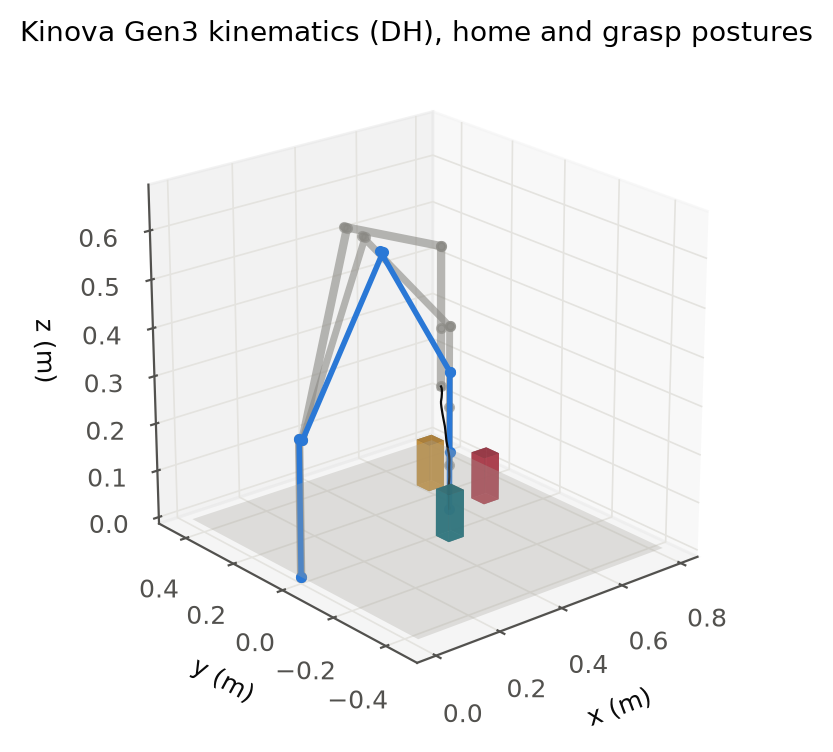
\includegraphics[width=0.85\columnwidth]{figures/arm_3d.png}
\caption{The simulated arm: Kinova Gen3 7-DoF kinematics from the manufacturer's DH table, shown at the home posture (grey) and during a DASA-assisted grasp (blue), with the tabletop scene and the TCP path.}
\label{fig:arm}
\end{figure}

\paragraph{Scene.} Three box objects (five in the \emph{clutter} scene) are placed at
least 12\,cm apart (8\,cm in clutter) on a $34\times60$\,cm table region. Each has a
random grasp yaw.

\paragraph{User.} The simulated user sees the scene with a 200\,ms visuomotor
delay~\cite{willett2017feedback}. It commands a top-down reach toward its goal, aligns
the wrist, opens the gripper while travelling, and closes it once at the grasp pose.
Its intent is expressed in decoder units with additive noise.

\paragraph{Command mapping.} Decoded $t_{x,y,z}$ map to TCP velocity at 0.08\,m/s per
unit, $r_x$ to yaw rate, and the mean of $g_{1..3}$ to gripper rate.

\paragraph{Grasp rule.} A grasp succeeds if the gripper closes with the TCP within
3\,cm of the goal's grasp point and the yaw within $20^\circ$. Closing on another
object is a \emph{wrong grasp}. Episodes time out after 20\,s.

\paragraph{Change of mind.} The user switches to another object after covering 70\% of
the distance to the first goal, by which point assistance is committed.

\paragraph{Arm.} We use the Kinova Gen3 7-DoF classical DH table~\cite{kinova2022gen3guide}
plus a 12\,cm gripper TCP. Control is resolved-rate damped least squares, with a
tool-down orientation task, a commanded yaw and a null-space posture term:
\begin{equation}
\dot q=J^\top(JJ^\top+\lambda^2I)^{-1}\xi+(I-J^+J)\,k_n(q_{\text{home}}-q).
\end{equation}
Every method's command passes through the same \emph{safety filter}:
\begin{itemize}
\item workspace box and table plane;
\item 0.2\,m/s speed cap;
\item joint-speed scaling and joint limits;
\item a link--table clearance check that blocks motions moving any joint origin
  further below 5\,cm.
\end{itemize}
Constraint activations are logged.

\subsection{Goal inference}
\paragraph{MaxEnt baseline}~\cite{ziebart2008maximum,dragan2013policy,javdani2015shared}.
For the decoded translation velocity $\hat u$ at TCP position $x$, distance cost and
look-ahead $h=0.5$\,s:
\begin{equation}
\log p(\hat u\mid g,x)=-\beta\big(\|\hat u\|h+d(x{+}\hat uh,g)-d(x,g)\big).
\end{equation}
$\beta$ is tuned per method.

\paragraph{Decoder-aware likelihood (DASA).} The open-loop calibration block gives
paired intended and decoded velocities. From these we fit the decoder error model
\begin{equation}
\hat z=G z^*+e,\qquad e\sim\mathcal N(0,\Sigma).
\end{equation}
We also measure the errors' integrated autocorrelation time
$\tau=1+2\sum_k\rho_k$, which is about 20 ticks for our smoothed decoder. Let
$z^*_g(x)$ be the user model's intended velocity toward goal $g$. Then
\begin{equation}
\log p(\hat z_t\mid g,x_t)=-\frac{1}{2\tau}\,r_g^\top\Sigma^{-1}r_g,\qquad r_g=\hat z_t-Gz^*_g(x_t).
\end{equation}
Dividing by $\tau$ counts correlated errors once per effective sample; without it the
posterior is over-confident. The likelihood uses all 7 decoded dimensions,
\emph{including wrist and grasp}, not only translation. It has no free temperature.

\paragraph{Switching prior.} Both DASA's inference and the ``+switching'' ablations use
an HMM forward recursion with hazard $\varepsilon=0.002$ per tick:
\begin{equation}
b_t(g)\propto p(\hat z_t\mid g,x_t)\big[(1-\varepsilon)b_{t-1}(g)+\varepsilon/K\big].
\end{equation}

\subsection{Arbitration}
All methods blend toward an autonomous reach policy $\pi_g$ (the same top-down
controller, using known object poses) or add to the user's command.
\begin{itemize}
\item \textbf{Decoder only:} $\alpha=0$.
\item \textbf{Fixed blend:} constant $\alpha$ toward the MAP goal.
\item \textbf{Distance blend}~\cite{downey2016blending}: autonomy weight
  $1-(1+e^{-aD+o})^{-1}$ with $a=11.6$ and $o=6.9$ (their constants). $D$ is the
  distance to the nearest object's grasp point divided by an envelope radius, and
  assistance goes toward that object.
\item \textbf{Confidence blend}~\cite{dragan2013policy}:
  $\alpha=\alpha_{\max}\,\mathrm{clip}\big((b_{\max}-0.4)/0.5,0,1\big)$.
\item \textbf{Hindsight assist}~\cite{javdani2015shared}: the robot adds the action
  minimising the posterior-expected cost-to-go,
  \begin{equation}
  a^*=\arg\min_a\sum_g b(g)\,\|x+(\hat u+a)h-t_g\|+\lambda\|a\|^2 ,
  \end{equation}
  where $t_g$ is where $\pi_g$ would lead. The problem is solved with Weiszfeld
  iterations. Yaw and grip receive the posterior-weighted correction.
\item \textbf{DASA:} the confidence ramp with the decoder-aware switching posterior,
  multiplied by a \emph{consistency gate}
  $\sigma\big((c_0-\bar m_t)/s\big)$. Here $\bar m_t$ is an exponential moving average
  (0.5\,s) of $r_{g^*}^\top\Sigma^{-1}r_{g^*}/7$, which is about 1 when the decoded
  commands are explained by the assisted goal and grows when the user pushes against
  it. This is innovation monitoring in the decoder's own noise units.
\end{itemize}

\paragraph{Fair tuning.} Each method's main hyper-parameters are tuned on separate
seeds at the nominal level:
\begin{itemize}
\item $\alpha$ and $\beta$ for fixed blending; $\beta$ for confidence blending;
  $\lambda$ and $\beta$ for hindsight; the envelope for distance blending; $c_0$ for DASA;
\item the objective is success $-$ wrong grasps $-\,0.01\times$time, over a 50/50 mix
  of standard and change-of-mind episodes.
\end{itemize}
The evaluation runs use paired scenes and noise seeds across methods, so we report
exact McNemar tests on paired successes.

%======================================================================
\section{Results: decoding}\label{sec:dec-results}
%======================================================================
\begin{table*}[t]
\centering\small
\adjustbox{max width=\textwidth}{\begin{tabular}{l c ccccccc}
\toprule
Decoder & R$^2_{\mathrm{vw}}$ & \texttt{tx} & \texttt{ty} & \texttt{tz} & \texttt{rx} & \texttt{g1} & \texttt{g2} & \texttt{g3} \\
\midrule
Wiener filter, global norm. & 0.319 & 0.17 & 0.02 & 0.15 & 0.34 & 0.42 & 0.32 & 0.25 \\
Wiener filter & 0.321 & 0.18 & 0.03 & 0.17 & 0.34 & 0.42 & 0.33 & 0.25 \\
Kalman filter & 0.242 & 0.17 & 0.08 & 0.18 & 0.33 & 0.35 & 0.23 & 0.13 \\
GRU & 0.626{\scriptsize$\pm$0.002} & 0.30 & 0.25 & 0.32 & 0.51 & 0.74 & 0.65 & 0.56 \\
Causal Transformer & 0.578 & 0.31 & 0.26 & 0.34 & 0.54 & 0.72 & 0.55 & 0.49 \\
Multi-day GRU, no aug. & 0.559 & 0.20 & 0.04 & 0.30 & 0.38 & 0.74 & 0.57 & 0.48 \\
\textbf{Multi-day GRU (ours)} & 0.574{\scriptsize$\pm$0.000} & 0.20 & 0.07 & 0.24 & 0.39 & 0.73 & 0.58 & 0.53 \\
\bottomrule
\end{tabular}
}
\caption{Within-session decoding on FALCON H1 held-in minival blocks (13 blocks, 6 days). R$^2_{\mathrm{vw}}$ is FALCON's variance-weighted R$^2$, averaged over blocks ($\pm$: std over seeds; 2 seeds for GRU and multi-day GRU). Per-DoF columns give R$^2$ pooled over blocks. For reference, FALCON reports held-in R$^2$ on its private test split of 0.24 (Wiener filter), 0.51 (RNN) and 0.68 (NDT2 Multi)~\cite{karpowicz2024falcon}; those values are not directly comparable to ours.}
\label{tab:within}
\end{table*}

\paragraph{Within session.}
\begin{itemize}
\item \textbf{Recurrent models dominate linear decoders} (Table~\ref{tab:within}, Fig.~\ref{fig:within}). The GRU reaches R$^2$=\GRUWithin{}, against \WienerWithin{} for the Wiener filter and \KalmanWithin{} for the Kalman filter.
\item \textbf{Per-DoF pattern.} The pooled per-DoF R$^2$ shows the same pattern for every decoder: grasp dimensions and wrist roll are decoded far better than translation, and $t_y$ is the hardest. The FALCON metric is variance-weighted, so it is dominated by the well-decoded grasp dimensions; a decoder that is good on the metric can still be poor at moving the hand in space. This is one reason we put the robot's assistance on translation and alignment.
\item \textbf{Multi-day GRU} (R$^2$=\MSGRUWithin): per-day read-ins slightly \emph{hurt} within-session accuracy relative to a single shared read-in. The extra $6\times$ input parameters overfit 2{,}300\,s of training data; its training loss ended well below the GRU's while its validation loss stayed higher.
\end{itemize}

\begin{figure*}[t]
\centering
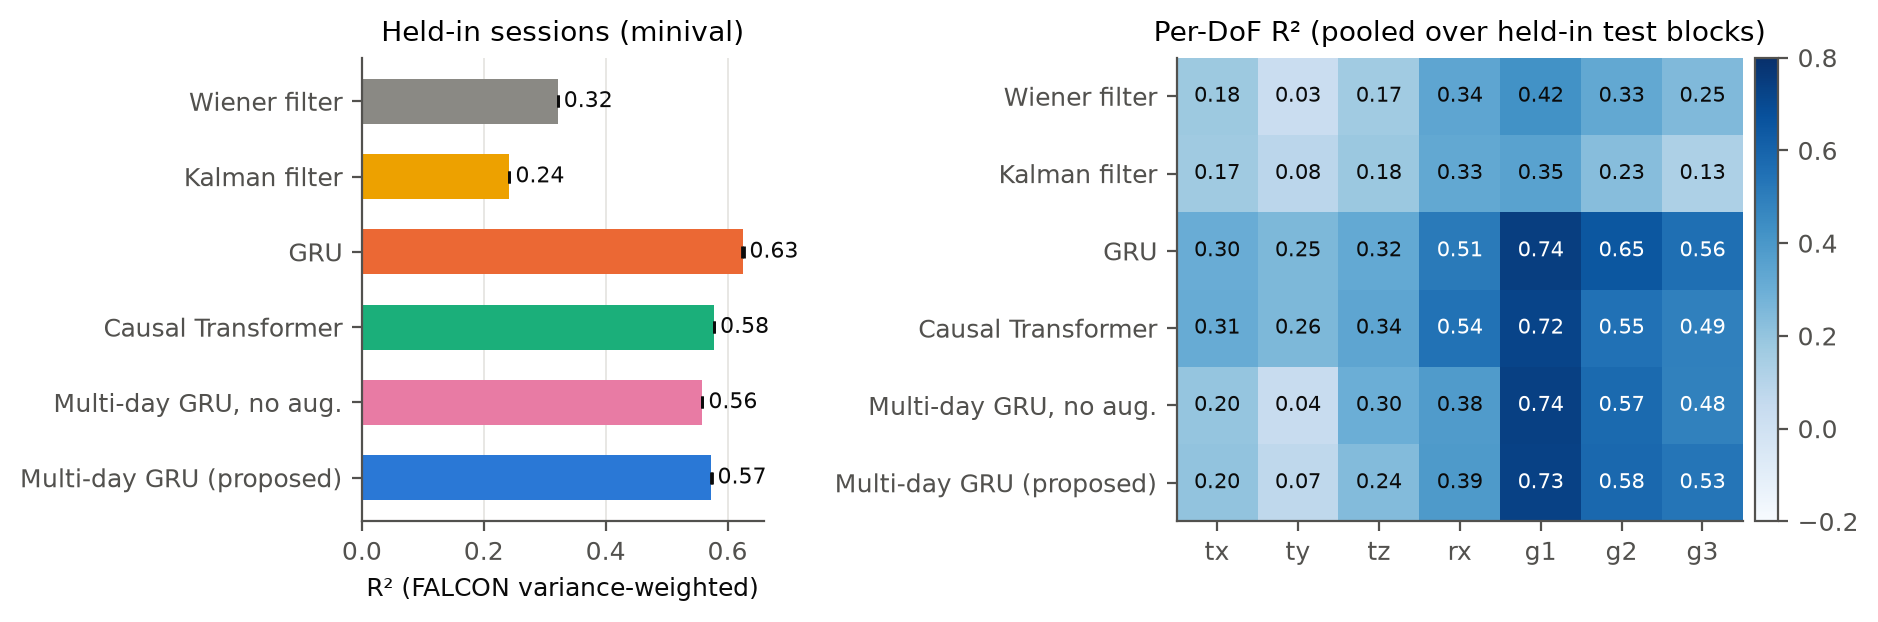
\includegraphics[width=0.9\textwidth]{figures/decoding_within.png}
\caption{Held-in decoding: variance-weighted R$^2$ (left) and per-DoF R$^2$ (right).}
\label{fig:within}
\end{figure*}

\begin{table*}[t]
\centering\small
\adjustbox{max width=\textwidth}{\begin{tabular}{l c ccc}
\toprule
& zero-shot & 10\,s & 20\,s & 45\,s \\
\midrule
Wiener filter, global norm. & 0.048 & -- & -- & -- \\
Wiener filter, held-in + new & 0.110 & 0.115 & 0.116 & 0.122 \\
Wiener filter, new data only & -- & -0.121 & 0.002 & 0.035 \\
Kalman filter & 0.039 & -- & -- & -- \\
GRU, fine-tune all & 0.247{\scriptsize$\pm$0.022} & 0.116{\scriptsize$\pm$0.006} & 0.160{\scriptsize$\pm$0.023} & 0.238{\scriptsize$\pm$0.047} \\
Causal Transformer, fine-tune all & 0.286 & 0.079 & 0.189 & 0.265 \\
Multi-day GRU, fine-tune all & 0.107{\scriptsize$\pm$0.078} & 0.217 & 0.198 & 0.222 \\
Multi-day GRU no aug., new read-in & 0.227 & 0.277 & 0.294 & 0.271 \\
\textbf{Multi-day GRU, new read-in (ours)} & 0.107{\scriptsize$\pm$0.078} & 0.272{\scriptsize$\pm$0.053} & 0.266{\scriptsize$\pm$0.049} & 0.285{\scriptsize$\pm$0.036} \\
\bottomrule
\end{tabular}
}
\caption{Cross-session decoding: R$^2_{\mathrm{vw}}$ on 7 later days (6--20 days after training), tested on block~B. Columns give the labelled seconds of the same day's block~A used for recalibration. All rows normalise inputs per day from block~A without labels, except ``global norm.'' This is our protocol, not FALCON's private split.}
\label{tab:cross}
\end{table*}

\paragraph{Across days.} Every decoder degrades on later days (Table~\ref{tab:cross}, Fig.~\ref{fig:cross}).
\begin{itemize}
\item \textbf{Normalisation.} Per-day z-scoring from unlabelled data is itself worth about 0.06 R$^2$ for the Wiener filter (\WienerZS{} vs \WienerGlobalZS{} with global normalisation).
\item \textbf{Zero-shot.} Neural decoders transfer better than linear ones. The single-read-in causal Transformer (0.286) and GRU (0.247) are the best zero-shot decoders. The multi-day GRU with an \emph{averaged} read-in is poor and unstable across seeds (\MSGRUZS$\pm$0.078), because the mean of day-specific read-ins is not itself a trained read-in.
\item \textbf{Full fine-tuning on seconds of data is harmful.} The GRU and the Transformer fine-tuned end-to-end on 10\,s fall far \emph{below} their own zero-shot accuracy (0.116 and 0.079), and recover only partly at 45\,s. A Wiener filter trained only on the new seconds is near or below zero.
\item \textbf{Read-in-only recalibration is the only adaptation that never hurts.} Fitting only a new input layer for the frozen multi-day core lifts it from \MSGRUZS{} to 0.27 with 10\,s and \MSGRUFew{} with \RecalMax\,s. At every budget this beats every other recalibration strategy: \GRUFew{} for the fine-tuned GRU at \RecalMax\,s, and \WienerPooledFew{} for the refit Wiener filter.
\item \textbf{The honest bottom line.} It does \emph{not} beat the best zero-shot model, the causal Transformer, by a meaningful margin. At this data scale (2{,}300\,s of training data, 6 days) the main benefit of read-in recalibration is robustness, since it never collapses, rather than higher accuracy than a well-regularised zero-shot decoder.
\item \textbf{Augmentation.} Removing the nonstationarity augmentation did not hurt few-shot accuracy here (single seed); we do not claim a benefit from it at this scale.
\end{itemize}
The absolute numbers (R$^2\approx0.2$--0.3 across days) underline how far 7-DoF decoding is from ``solved'' at this data scale, and motivate the shared autonomy below.

\begin{figure*}[t]
\centering
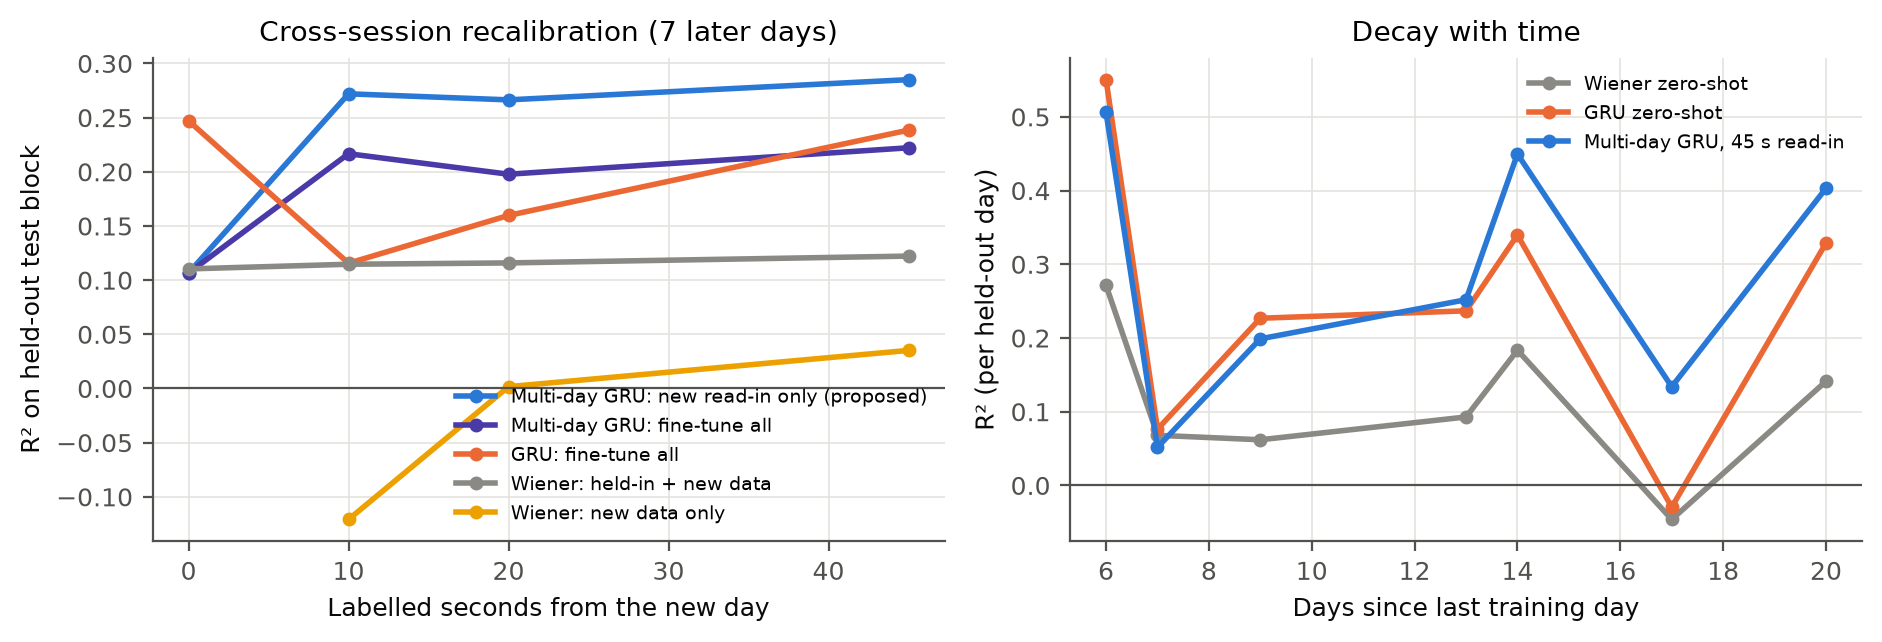
\includegraphics[width=0.9\textwidth]{figures/decoding_cross_session.png}
\caption{Cross-session recalibration (left) and per-day R$^2$ against days since the last training day (right).}
\label{fig:cross}
\end{figure*}

\begin{figure*}[t]
\centering
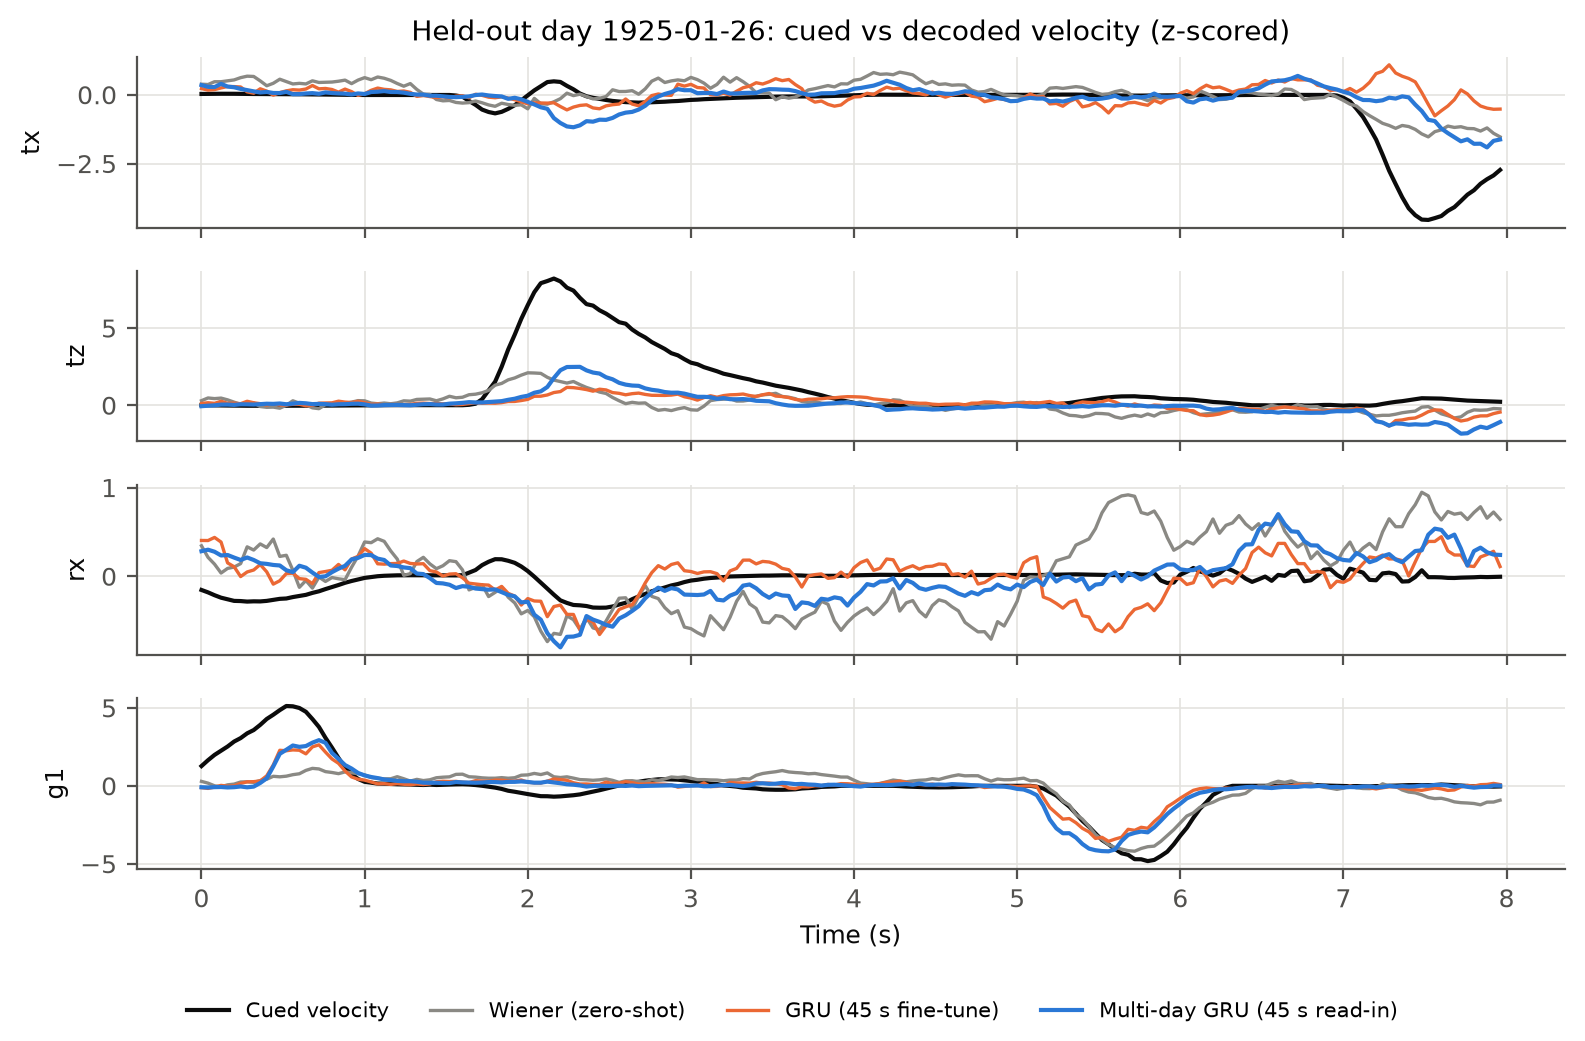
\includegraphics[width=0.8\textwidth]{figures/decoding_traces.png}
\caption{Cued (black) and decoded velocity on a held-out day, in z-scored units, for four of the seven DoF: zero-shot Wiener filter, GRU fine-tuned on 45\,s, and multi-day GRU with a 45\,s read-in. Translation ($t_x$, $t_z$) is decoded far less faithfully than wrist roll and grasp.}
\label{fig:traces}
\end{figure*}


%======================================================================
\section{Results: shared autonomy in the simulated closed loop}
%======================================================================
\paragraph{Anchoring the simulator.} The decoder-quality dial is anchored to two real reference points:
\begin{itemize}
\item A Wiener filter with FALCON's 600\,ms history, trained on all held-in days, reaches R$^2$=\RealRsqMulti{} on real minival data. The nominal level is the dial setting whose simulated R$^2$ is closest to this value: \NominalRsq{} at $\kappa=\NominalKappa$.
\item The closed-loop decoder itself (10 taps, one session) reaches only \RealRsq{} on real data, at the low end of the dial.
\end{itemize}
Results at the nominal level use \Episodes{} paired episodes per method and scenario.

\begin{table*}[t]
\centering\small
\adjustbox{max width=\textwidth}{\begin{tabular}{l ccccc ccc cc}
\toprule
& \multicolumn{5}{c}{Standard (3 objects)} & \multicolumn{3}{c}{Change of mind} & \multicolumn{2}{c}{Clutter (5 obj.)} \\
\cmidrule(lr){2-6}\cmidrule(lr){7-9}\cmidrule(lr){10-11}
Method & Succ. & Wrong & Time (s) & Path eff. & User share & Succ. & Wrong & Yield (s) & Succ. & Wrong \\
\midrule
Decoder only & 0.02 & 0.00 & 19.0 & 0.17 & 1.00 & 0.05 & 0.00 & 3.24 & 0.05 & 0.00 \\
Fixed blend & 0.88 & 0.02 & 6.9 & 0.69 & 0.29 & 0.88 & 0.07 & 2.66 & 0.75 & 0.02 \\
Distance blend [Downey'16] & 1.00 & 0.00 & 8.3 & 0.51 & 0.76 & 0.47 & 0.45 & 3.00 & 0.93 & 0.07 \\
Confidence blend [Dragan'13] & 0.90 & 0.00 & 7.2 & 0.66 & 0.24 & 0.92 & 0.07 & 2.26 & 0.78 & 0.02 \\
Hindsight assist [Javdani'15] & 0.90 & 0.02 & 6.8 & 0.67 & 0.49 & 0.68 & 0.23 & 2.61 & 0.70 & 0.02 \\
\textbf{DASA (ours)} & 1.00 & 0.00 & 5.2 & 0.83 & 0.29 & 1.00 & 0.00 & 0.73 & 1.00 & 0.00 \\
\bottomrule
\end{tabular}
}
\caption{Simulated closed loop at the nominal decoder quality (offline R$^2$=\NominalRsq). \emph{Wrong}: closed the gripper on a non-goal object. \emph{Time} and \emph{path efficiency} are over successful episodes. \emph{User share}: the user's share of the command norm. \emph{Yield}: median time from the change of mind until the goal estimate settles on the new goal. Hyper-parameters of every method were tuned on separate seeds.}
\label{tab:sa}
\end{table*}

\begin{figure*}[t]
\centering
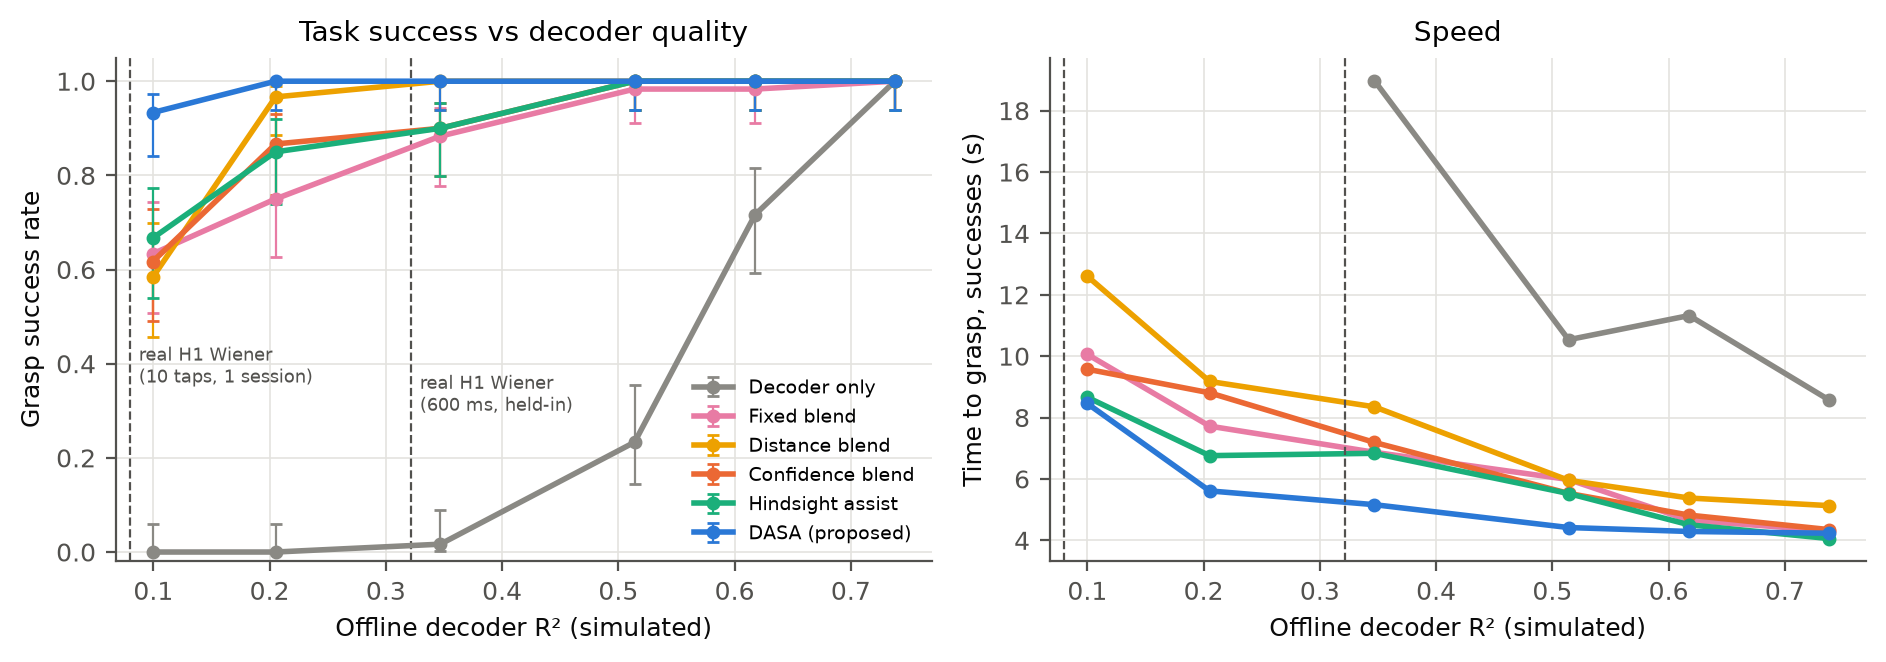
\includegraphics[width=0.85\textwidth]{figures/success_vs_r2.png}
\caption{Success and time-to-grasp against simulated offline decoder R$^2$ (Wilson 95\% CIs; 60 episodes per point). Dashed lines mark two real-data references: the closed-loop decoder configuration on its own session, and a FALCON-style Wiener filter on held-in data.}
\label{fig:sweep}
\end{figure*}

\paragraph{Assistance is necessary at today's decoding accuracy.}
\begin{itemize}
\item \textbf{Decoder only.} Without assistance the simulated user grasps the goal in \SuccDirect{} of standard episodes at the nominal level (Table~\ref{tab:sa}). The arm still reaches the vicinity of the goal; what fails is the final 3\,cm/20$^\circ$ alignment and a clean gripper closure. Decoder-only success needs offline R$^2\gtrsim0.6$ to exceed 50\% (Fig.~\ref{fig:sweep}).
\item \textbf{Every assisted method} raises success to 0.88--1.00 at the nominal level. This matches the clinical observation that shared control rescues grasping~\cite{downey2016blending}.
\end{itemize}

\paragraph{DASA is faster, straighter and never grasps the wrong object.}
On the standard task:
\begin{itemize}
\item DASA succeeds in \SuccDASA{} of episodes and grasps in \TimeDASA\,s on average, versus \TimeConfidence\,s for confidence blending and \TimeHindsight\,s for hindsight assistance.
\item Its path efficiency is the highest of all methods.
\item Its paired success advantage is significant over fixed blending (McNemar $p$=\PStdFixed), confidence blending ($p$=\PStdConfidence) and hindsight assistance ($p$=\PStdHindsight).
\item Distance blending also reaches \SuccDistance{}, but is slower (\TimeDistance\,s), because assistance only switches on inside the grasp envelope.
\end{itemize}
DASA's goal estimate is correct earlier in the episode than any baseline's (Fig.~\ref{fig:goal}). The reason: its likelihood uses all seven decoded dimensions, wrist and grasp included, and it weights them by their measured reliability.

\paragraph{Clutter.} With five objects at least 8\,cm apart:
\begin{itemize}
\item MaxEnt-based methods drop to \ClutSuccConfidence{} (confidence blending) and \ClutSuccHindsight{} (hindsight).
\item Distance blending holds up at \ClutSuccDistance{}, but grasps the wrong object in \ClutWrongDistance{} of episodes.
\item DASA keeps \ClutSuccDASA{} success with no wrong grasps.
\end{itemize}

\begin{figure}[t]
\centering
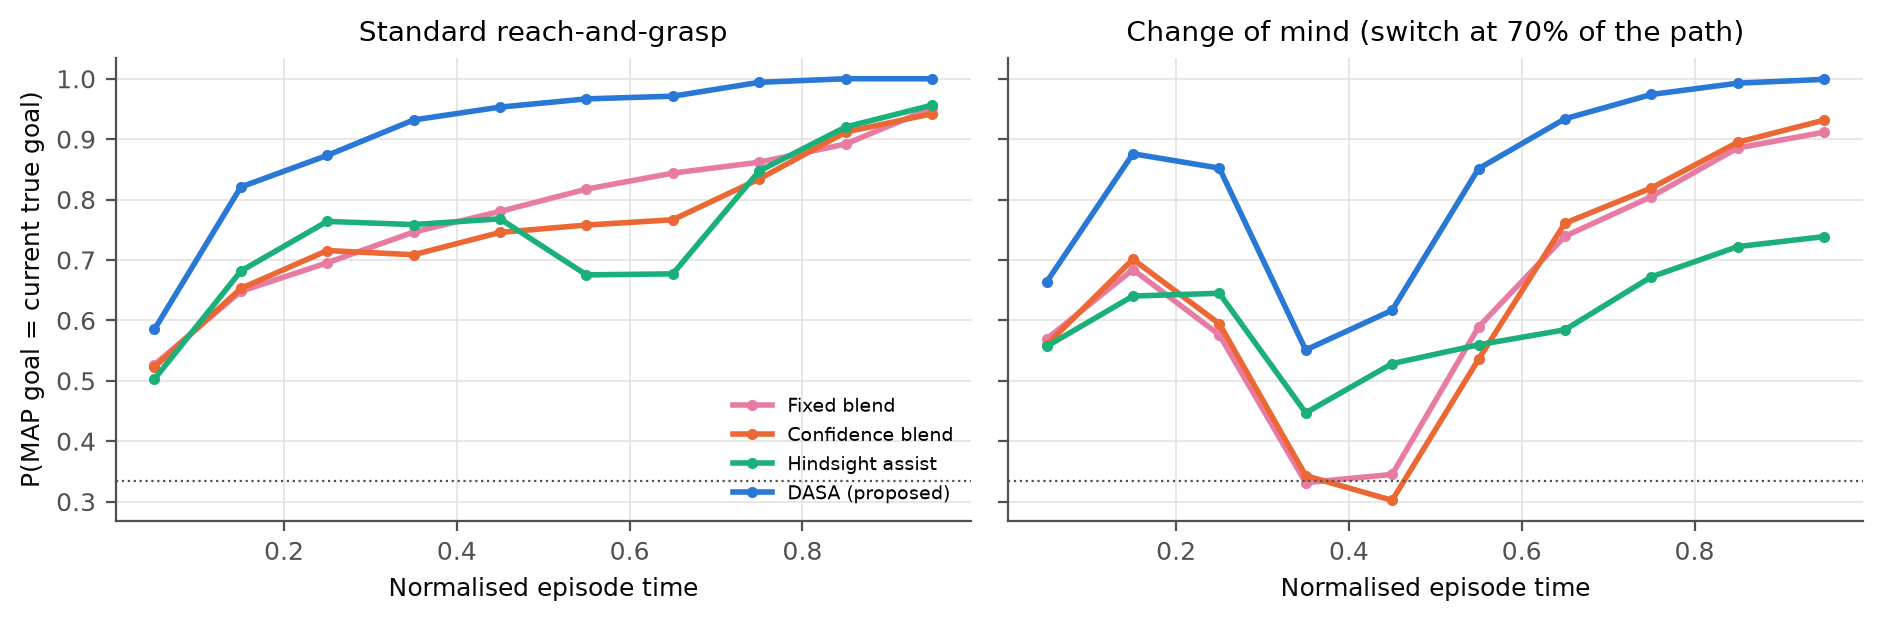
\includegraphics[width=\columnwidth]{figures/goal_inference.png}
\caption{Probability that the MAP goal equals the user's current goal over normalised episode time (nominal decoder). Dotted line: chance with three objects.}
\label{fig:goal}
\end{figure}

\paragraph{Changing one's mind: assistance must yield.}
In this scenario the user switches goals after covering 70\% of the way to the first object, by which point every method's assistance is committed.
\begin{itemize}
\item \textbf{Distance blending} is the worst. It assists toward whichever object is nearest, so it grasps the abandoned object in \ComWrongDistance{} of episodes.
\item \textbf{Hindsight assistance} also grasps the wrong object in \ComWrongHindsight{} of episodes. Its accumulated posterior keeps pulling the arm toward the first goal.
\item \textbf{DASA} settles on the new goal after a median of \YieldDASA\,s, versus \YieldConfidence\,s for confidence blending and \YieldHindsight\,s for hindsight. It succeeds in \ComSuccDASA{} of change-of-mind episodes with no wrong grasps (Fig.~\ref{fig:com}).
\end{itemize}
The ablations (below) show that the switching prior and the calibrated likelihood are what make this fast yielding possible.

\begin{figure*}[t]
\centering
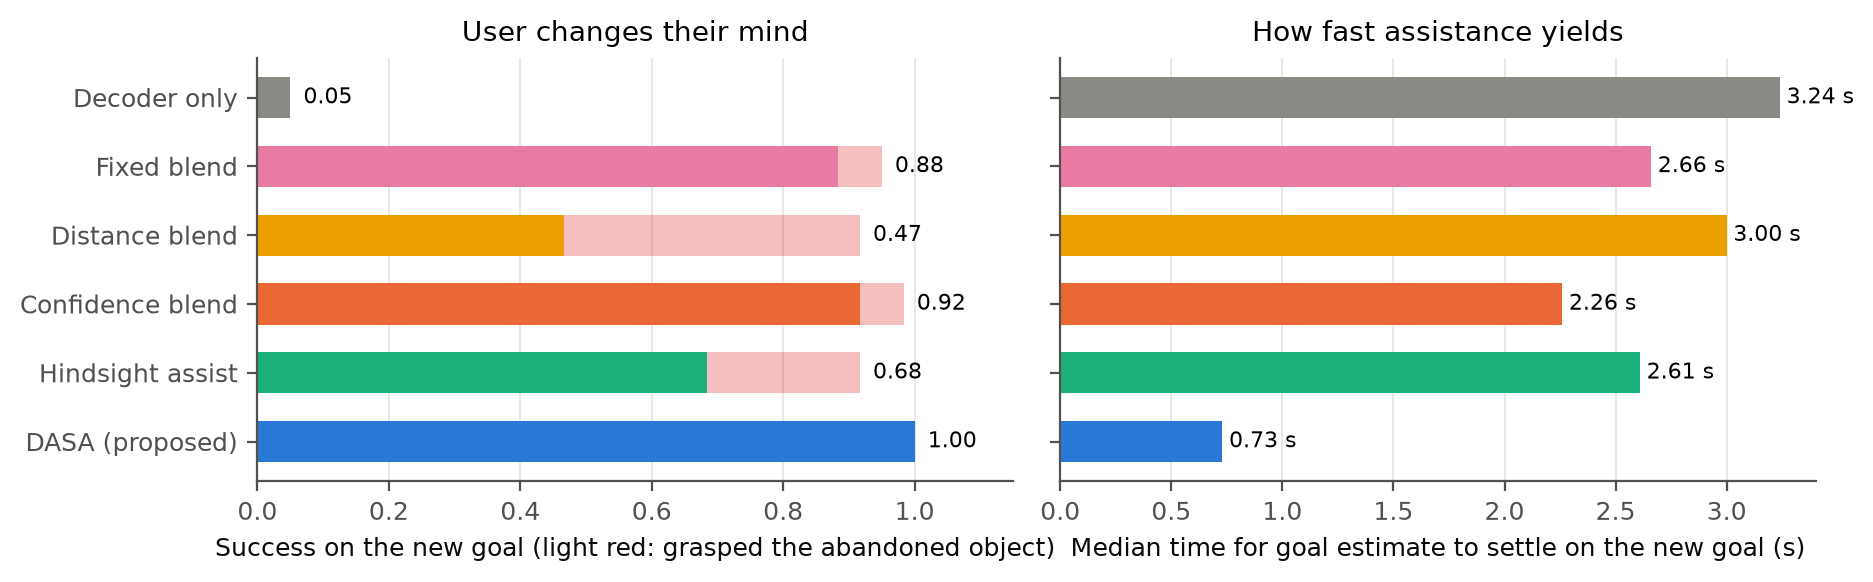
\includegraphics[width=0.85\textwidth]{figures/change_of_mind.png}
\caption{Change-of-mind scenario at the nominal decoder. Left: success on the new goal; shaded red marks episodes that closed on the abandoned object. Right: median yield latency.}
\label{fig:com}
\end{figure*}

\paragraph{Authority versus performance.}
Success can always be bought by taking control away from the user, so we sweep each method's assistance strength (Fig.~\ref{fig:authority}).
\begin{itemize}
\item At a user share of about 0.5, DASA ($\alpha_{\max}=0.6$) is still at ceiling success. Confidence and fixed blending at a similar share succeed in only 0.57--0.64 of episodes.
\item Hindsight assistance, which by construction keeps the user's command and adds a correction, sits near a 0.5 share at 0.80--0.83 success.
\end{itemize}
DASA therefore offers a strictly better frontier in this simulation: it can return half of the control to the user without losing success. This matters because users value authority~\cite{javdani2015shared,gopinath2017human}.

\begin{figure*}[t]
\centering
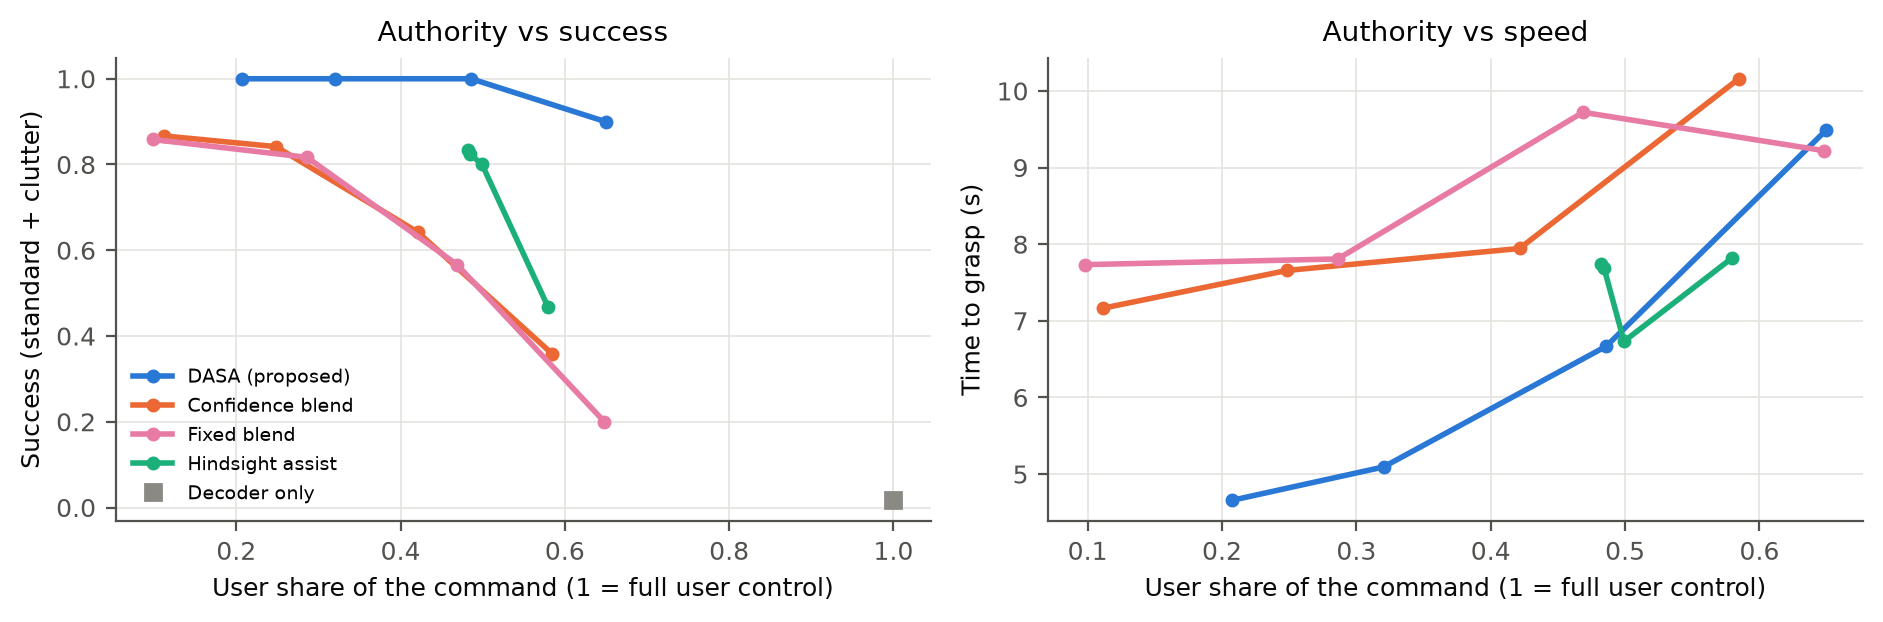
\includegraphics[width=0.85\textwidth]{figures/authority_tradeoff.png}
\caption{Authority--performance trade-off at the nominal decoder (standard + clutter episodes). Each method's assistance strength is swept: $\alpha_{\max}$ for DASA and confidence blending, $\alpha$ for fixed blending, $\lambda$ for hindsight assistance. Upper right is better.}
\label{fig:authority}
\end{figure*}

\paragraph{Ablations.} Table~\ref{tab:abl} and Fig.~\ref{fig:abl} report the ablations at the nominal level and at the weakest decoder (R$^2\approx0.1$). At the nominal level DASA saturates, so most differences there appear as slower yielding rather than as lost successes.
\begin{itemize}
\item \textbf{Autocorrelation correction} is the most important component. Without it the posterior becomes over-confident on correlated decoder errors. At the weakest decoder, success falls from 0.93/0.85/0.87 (standard / change of mind / clutter) to 0.70/0.47/0.27. At the nominal level, yielding slows from 0.73\,s to 3.6\,s.
\item \textbf{The calibrated error model} ($G$, $\Sigma$, $\tau$ replaced by identity) is the next most important. At the weakest decoder, success falls to 0.77/0.63/0.68, and nominal yielding slows to 4.1\,s.
\item \textbf{The switching prior} matters for changes of mind. Without it, nominal yielding takes 2.5\,s; at the weakest decoder, change-of-mind success drops to 0.75 and wrong grasps double (0.20 vs 0.10).
\item \textbf{The consistency gate} has no effect at the nominal level. At the weakest decoder it raises change-of-mind success from 0.73 to 0.85, at a negligible cost on the standard task.
\item \textbf{A user model with the wrong speed} (assumed 2$\times$ slower) costs little at the nominal level. At the weakest decoder, clutter success drops to 0.63.
\item \textbf{A switching prior on MaxEnt inference does not work}, even with its temperature re-tuned: success is 0.30 or lower. A MaxEnt likelihood is too weak and too poorly calibrated to overcome the switching hazard, so the posterior never concentrates. The switching prior is usable only with a likelihood calibrated to the decoder's noise.
\end{itemize}

\begin{table}[t]
\centering\scriptsize
\setlength{\tabcolsep}{3pt}
\adjustbox{max width=\columnwidth}{\begin{tabular}{l ccc ccc}
\toprule
& \multicolumn{3}{c}{Nominal (R$^2$ 0.35)} & \multicolumn{3}{c}{Weakest (R$^2$ 0.10)} \\
\cmidrule(lr){2-4}\cmidrule(lr){5-7}
Variant & Std. & Change & Clutter & Std. & Change & Clutter \\
\midrule
DASA (full) & 1.00 & 1.00 & 1.00 & 0.93 & 0.85 & 0.87 \\
$-$ consistency gate & 1.00 & 1.00 & 1.00 & 0.95 & 0.73 & 0.87 \\
$-$ switching prior & 1.00 & 0.97 & 1.00 & 0.93 & 0.75 & 0.88 \\
$-$ autocorrelation correction ($\tau{=}1$) & 1.00 & 0.98 & 0.97 & 0.70 & 0.47 & 0.27 \\
$-$ calibrated error model ($G{=}I,\Sigma{=}I,\tau{=}1$) & 1.00 & 1.00 & 1.00 & 0.77 & 0.63 & 0.68 \\
mismatched user model (speed $\times0.5$) & 1.00 & 0.98 & 1.00 & 0.83 & 0.80 & 0.63 \\
Confidence blend + switching prior & 0.10 & 0.03 & 0.07 & 0.00 & 0.02 & 0.02 \\
Confidence + switching, $\beta$ re-tuned & 0.30 & 0.35 & 0.20 & 0.02 & 0.02 & 0.00 \\
\bottomrule
\end{tabular}
}
\caption{Ablations: success rate (60 episodes per cell) at the nominal and the weakest simulated decoder.}
\label{tab:abl}
\end{table}

\begin{figure*}[t]
\centering
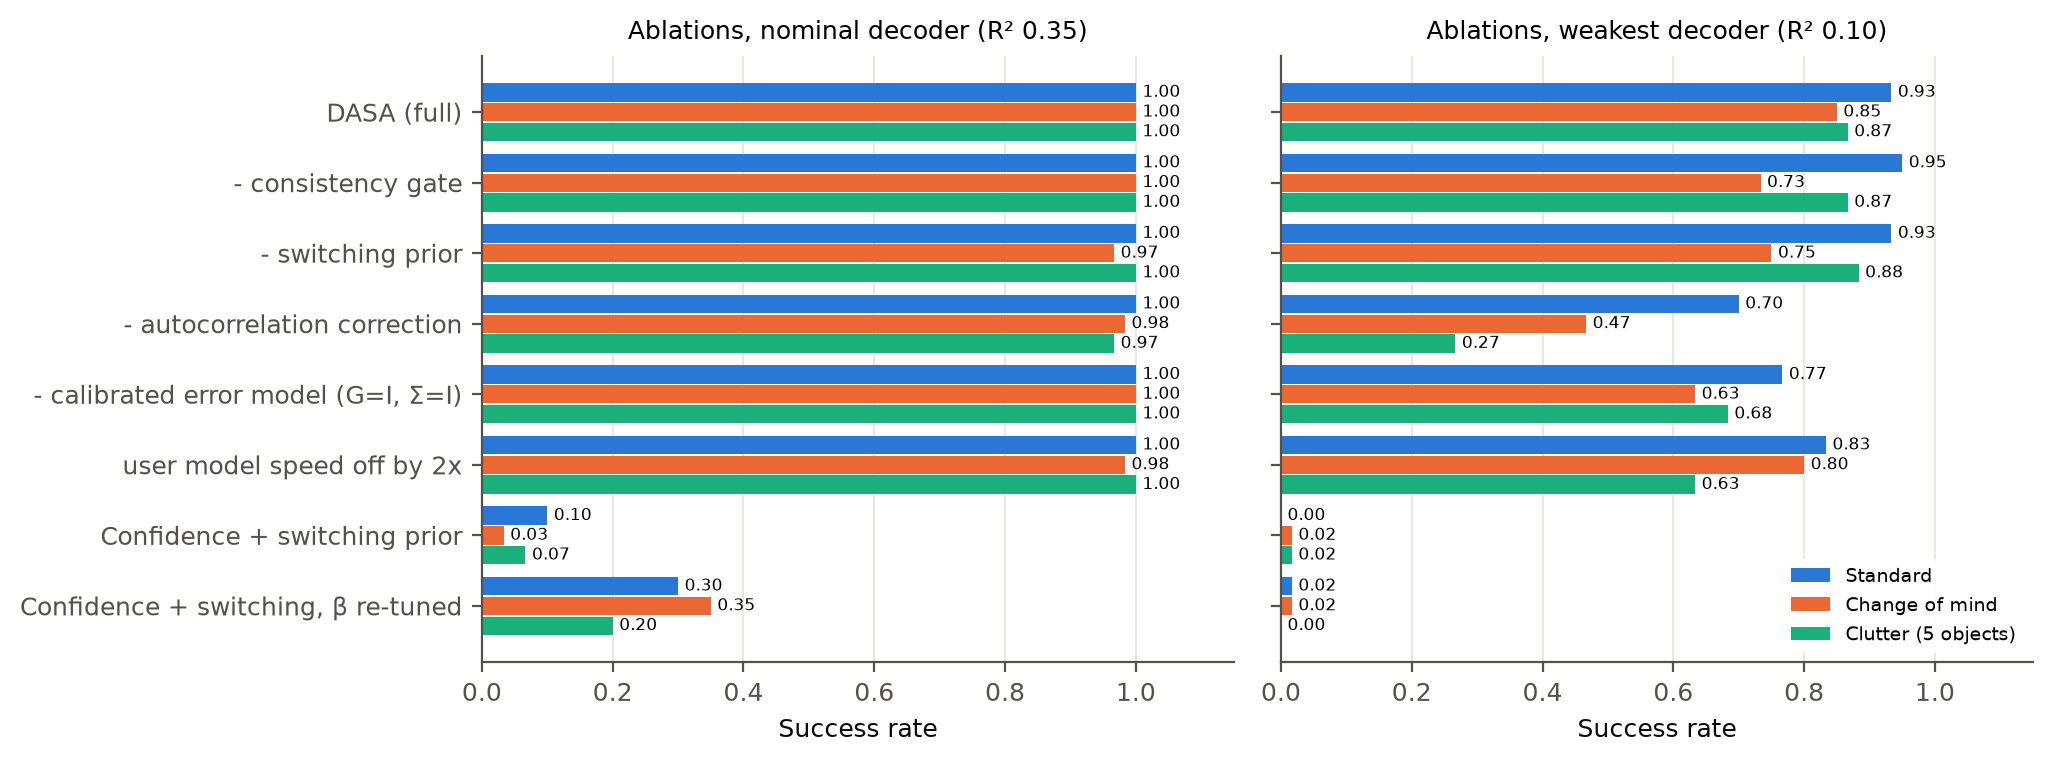
\includegraphics[width=0.9\textwidth]{figures/ablations.png}
\caption{Ablations of DASA, and MaxEnt inference with a switching prior.}
\label{fig:abl}
\end{figure*}

\paragraph{Safety filter.} The same safety filter is applied after every method.
\begin{itemize}
\item With assistance the speed cap rarely engages: about 0.1 times per episode for DASA at the nominal level, against about 15 per episode for the noisy decoder alone.
\item Across all \SafetyEpisodes{} simulated episodes of the run, the link--table check never had to block a motion (\SafetyLinkTable{} episodes). Joint-limit clipping occurred in \SafetyJointLimit{} episodes, workspace clipping in \SafetyWorkspace{}, and table-plane clipping in \SafetyTablePlane{} (mostly under decoder-only control).
\end{itemize}
Example trajectories are shown in Fig.~\ref{fig:episodes}.

\begin{figure*}[t]
\centering
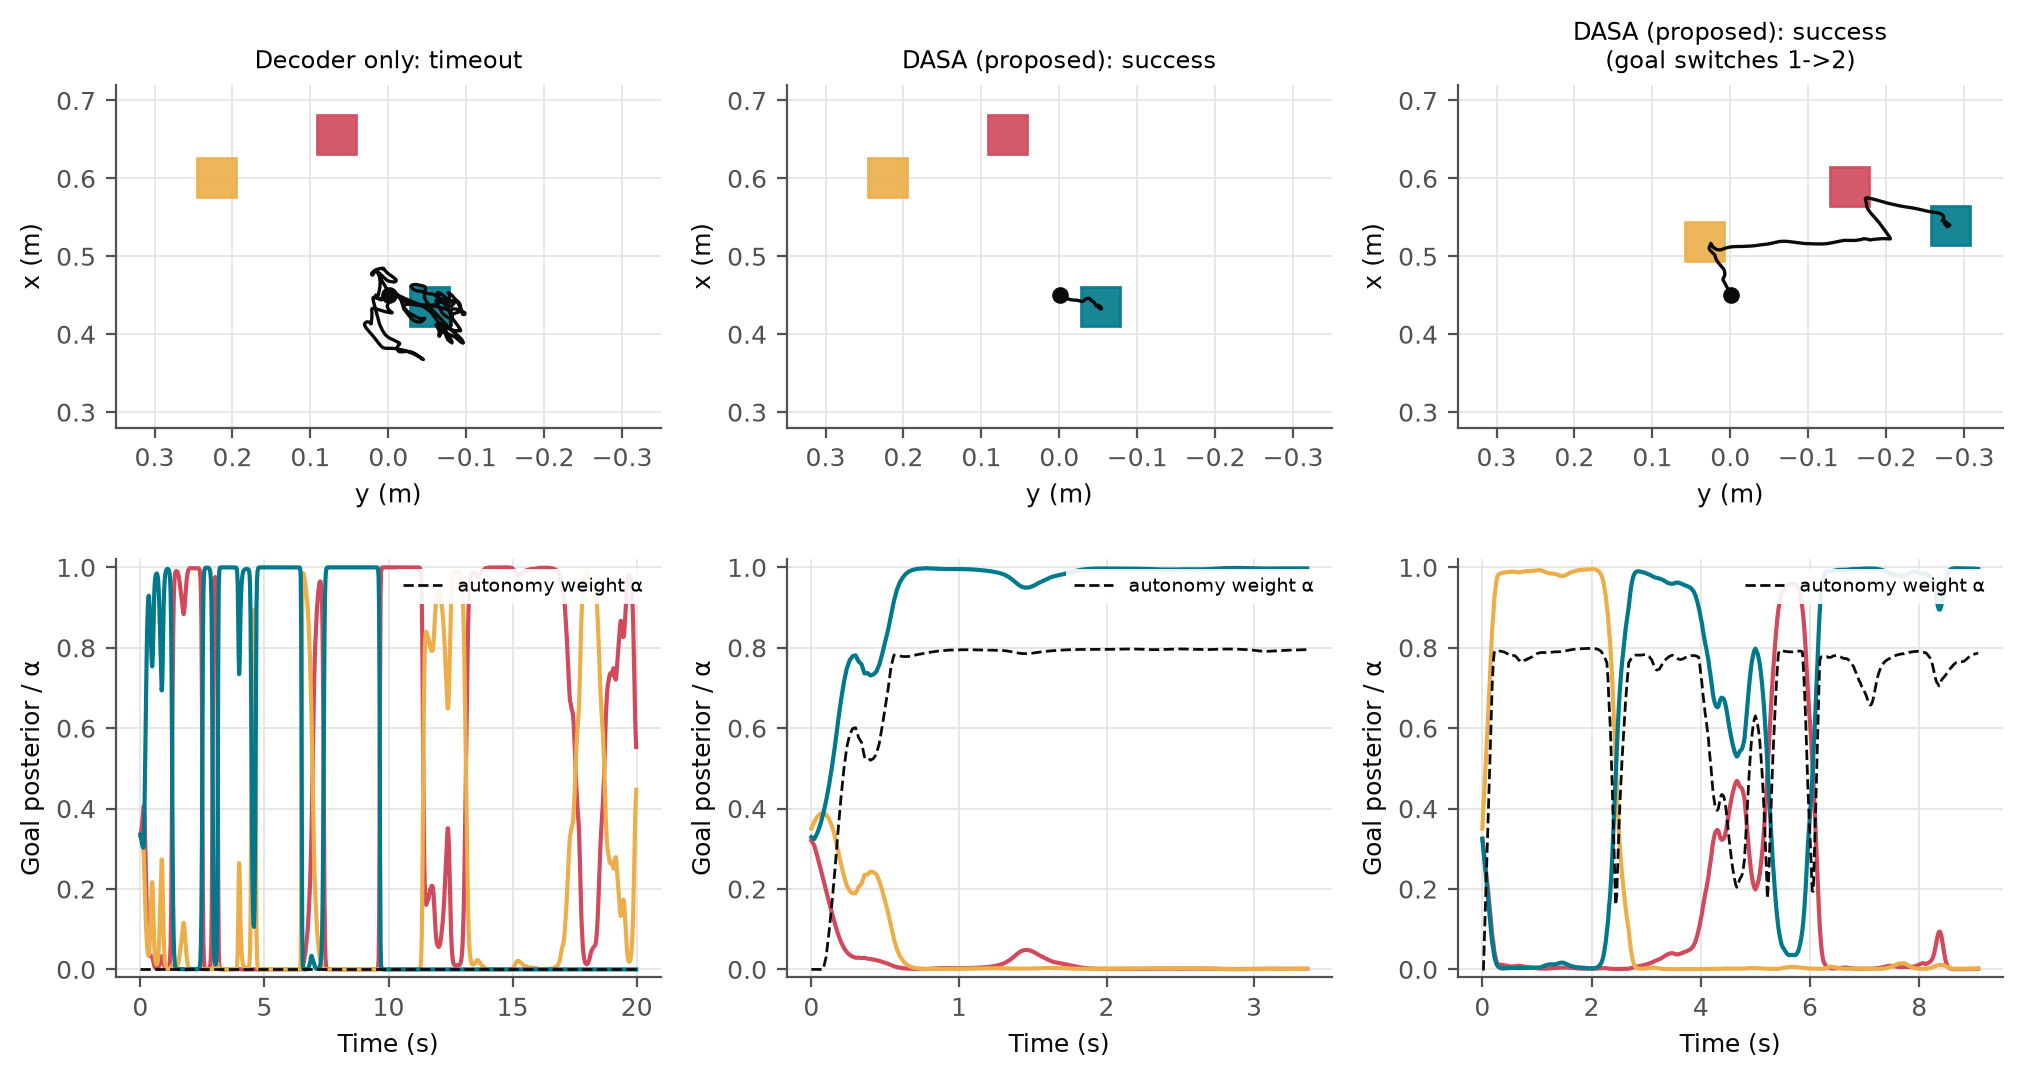
\includegraphics[width=0.78\textwidth]{figures/example_episodes.png}
\caption{Example episodes (top view; robot base at the origin, $x$ pointing away from the base). Left: decoder only on a scene where it times out. Middle: DASA on the same scene. Right: DASA with a change of mind. Bottom: goal posterior per object (object colours) and autonomy weight $\alpha$.}
\label{fig:episodes}
\end{figure*}


%======================================================================
\section{Discussion}
%======================================================================
\paragraph{What matters for a product.} The two halves of this study point the same way.

\begin{itemize}
\item \textbf{Offline accuracy on real H1 data is modest and decays across days.} The decoding results bear this out (\S\ref{sec:dec-results}).
\item \textbf{The decoder alone is far from enough at that accuracy.} In the simulated closed loop, decoder-only control almost never completes a 3\,cm/20$^\circ$ grasp until offline R$^2$ exceeds about 0.6.
\item \textbf{Assistance makes the task feasible at present-day accuracy.} Within assistance, \emph{how} the robot infers intent matters most when the scene is cluttered or the user changes their mind. Those are exactly the situations where a wrong grasp is costly.
\item \textbf{Calibrating the inference to the decoder is the useful idea.} In a BCI the user's command is the output of a decoder, so the inference should model that decoder. Its gain, covariance and autocorrelation are already measured during the open-loop calibration block that every clinical session starts with. Using them removes a hand-tuned temperature, lets wrist and grasp signals contribute evidence, and makes a goal-switching prior usable.
\end{itemize}

\paragraph{Decoder improvements and assistance are complementary.} Fig.~\ref{fig:sweep} turns offline R$^2$ into closed-loop success under our model. The gains of better decoders appear mostly in decoder-only and weak-assistance regimes; with DASA, success saturates early, and better decoders instead buy speed and authority. One practical reading for product decisions: at a given decoder quality, the assistance policy determines how much control can be handed back to the user without failures (Fig.~\ref{fig:authority}).

\paragraph{Recalibration cost.} Fitting only a per-day input layer suits daily recalibration of a deployed decoder. The trained core is fixed, so the decoder's behaviour stays predictable, and only a small, well-regularised layer changes. With seconds of data it is the only adaptation we tested that never made things worse. On H1 at this scale, however, its accuracy only matches a single-read-in Transformer used zero-shot. With more training days, which is the regime of NDT2/NDT3-style pretraining~\cite{ye2023neural,ye2025generalist}, we expect the multi-day core to benefit more. \texttt{configs/gpu.yaml} is set up to test this.

\paragraph{A data-handling pitfall.} The public FALCON H1 calibration files contain the minival segment, which is the first part of each calibration file, bin for bin. Training on them without removing it inflated our GRU's held-in R$^2$ to 0.80 (versus \GRUWithin{} after removal) in an earlier run, whose log is retained in the repository. The Wiener filter was inflated far less (0.38 versus \WienerWithin). All results reported here strip the overlap, and a unit test guards it.

\paragraph{Future work.}
\begin{itemize}
\item Human-in-the-loop evaluation, including user preference for authority.
\item Learned perception, so that goals are not given by known object poses.
\item Grasp physics.
\item Inferring goals over continuous targets, not only a discrete set of objects.
\item Closed-loop recalibration with intention relabelling~\cite{gilja2012high,wilson2025longterm}, using DASA's goal posterior as the relabelling signal.
\end{itemize}


%======================================================================
\section{Reproducing at full scale}\label{sec:repro}
%======================================================================
Every number here comes from \texttt{scripts/run\_cpu.sh} (\texttt{configs/cpu.yaml})
on a shared 8-core Intel CPU. The CPU budget constrains the experiments in three ways:
\begin{itemize}
\item decoders are small (a 1-layer GRU with 192 units, 1{,}200 steps);
\item we use 2 seeds for the GRU and the multi-day GRU, and 1 for the other neural
  variants;
\item the closed loop uses 60 episodes per cell.
\end{itemize}
\texttt{scripts/run\_gpu.sh} runs the same code with \texttt{configs/gpu.yaml} on a
fresh Linux CUDA machine. It creates a virtual environment, installs
\texttt{requirements-gpu.txt}, downloads FALCON H1 (102\,MB) and runs the full
pipeline: 2-layer 512-unit GRUs, 4-layer Transformers, 20k steps, 5 seeds, bfloat16
autocast, nine decoder-quality levels and 300 episodes per cell. All metrics,
figures, tables and website files are regenerated from the JSON results.

%======================================================================
\section{Limitations}
%======================================================================
\begin{itemize}
\item \textbf{No human in the loop.} The user model does not learn, adapt to the decoder
  or to assistance, fatigue, or express preferences. Javdani et
  al.~\cite{javdani2015shared} found users did not prefer the faster assistance policy,
  and real users co-adapt with decoders. Closed-loop results here are evidence about
  algorithms under a model, not about people.
\item \textbf{Model match favours DASA.} DASA's likelihood uses the structure of the
  simulated user's policy. Our mismatch ablation perturbs only speed. Perception is
  perfect (known object poses).
\item \textbf{Encoding model.} It is linear-Poisson in velocity with slow latents. It has
  no neural dynamics or goal/position tuning. The simulated R$^2$ is matched to the
  real R$^2$ for one decoder on one session.
\item \textbf{Kinematics only.} There is no grasp physics or object collision checking,
  the objects are boxes, and grasps are top grasps.
\item \textbf{Decoding evaluation.} Our cross-session protocol uses short test blocks
  (about 50\,s, 3 trials each) on 7 days and is not FALCON's private split. The CPU
  scale limits the neural decoders.
\end{itemize}

%======================================================================
\section{Broader impact and safety}
%======================================================================
Assistive arms act in physical space near a person who cannot move out of the way.
\begin{itemize}
\item The design choices emphasised here favour \emph{safety and user authority over
  raw speed}:
  \begin{itemize}
  \item a method-independent safety filter;
  \item explicit handling of changed intent;
  \item reporting of wrong-object grasps;
  \item reporting the user's share of the command, not only success.
  \end{itemize}
\item A shared-autonomy system that succeeds by taking over could reduce users' sense of
  agency. The authority/performance trade-off should be set with users, not for them~\cite{gopinath2017human}.
\item Simulation results must not be read as clinical efficacy.
\item The Kinova Gen3 user guide itself states that the robot is not intended for
  clinical assistive use. We use it only as a kinematic model.
\item This is an independent project, not affiliated with Neuralink.
\end{itemize}
